%%%%%%%%%%%%%%%%%%%%%%%%%%% COORDINATESYSTEMS
% COORDSYS (ORIGOCOORDINATENAME, WIDTH, HEIGHT)
% Draws a Coordinatesystem around ORIGOCOORDINATENAME with a width of WIDTH and a height of HEIGHT, 
% names the beginning and end of axes, southwest corner, northwest corner, 
\newcommand{\OneQuadrantCoordSys}[3]{
\coordinate (XY#1) at ([xshift=#2 cm, yshift=#3 cm]#1);
%\coordinate (-XY#1) at ([xshift=-#2 cm, yshift=-#3 cm]#1);
%\coordinate (-X#1) at ([xshift=-#2 cm]#1);
\coordinate (X#1) at ([xshift=#2 cm]#1);
\coordinate (Y#1) at ([yshift=#3 cm]#1);
%\coordinate (-Y#1) at ([yshift=-#3 cm]#1);
%\draw [help lines, step=.5cm] (#1) grid (XY#1);
\draw[->, name path=XAxis#1] (#1)--(X#1);
\draw[->, name path=YAxis#1] (#1)--(Y#1);
}

% \DistanceLabel{SS}{AS}{-45}{1}{pos=.5}{1}
\newcommand{\DistanceLabel}[6]{
\coordinate(#1horgony) at ([shift=(#3:#4)] #1);
\coordinate(#2horgony) at ([shift=(#3:#4)] #2);
\draw[thin, red, <->] (#1horgony)--(#2horgony) node[#5, scale=.7]{#6};
\draw[opacity=.4, black] (#1)--(#1horgony);
\draw[opacity=.4, black] (#2)--(#2horgony);
}

%Lorentz(OriginalOriginCoord, ResultingOriginCoord, SpeedNum, PointCoord, Label)
% 
\newcommand{\Lorentz}[5]{
\path (#1); \pgfgetlastxy{\XCoord}{\YCoord}; % Extracting coordinates of the Origin
\pgfmathsetmacro{\XOrigin}{\XCoord} % Saving X coordinate
\pgfmathsetmacro{\YOrigin}{\YCoord} % Saving Y coordinate
\path (#4); \pgfgetlastxy{\XCoord}{\YCoord}; % Extracting coordinates of the Point
\pgfmathsetmacro{\XEvent}{\XCoord} % Saving X coordinate
\pgfmathsetmacro{\YEvent}{\YCoord} % Saving Y coordinate
\pgfmathsetmacro{\XEventWRTOrigin}{\XEvent-\XOrigin} % Relativizing to the origin
\pgfmathsetmacro{\YEventWRTOrigin}{\YEvent-\YOrigin} % Relativizing to the origin
\pgfmathparse{XLorentz(#3,\XEventWRTOrigin,\YEventWRTOrigin)} % transforming x
\pgfmathsetmacro{\XEventTr}{\pgfmathresult} % save the result of x
\pgfmathparse{YLorentz(#3,\XEventWRTOrigin,\YEventWRTOrigin)} % transforming y
\pgfmathsetmacro{\YEventTr}{\pgfmathresult} % save the result of y
\node[inner sep=0](#5) at (
[xshift=\XEventTr pt,
 yshift=\YEventTr pt] #2){};
}

\usetikzlibrary{calc}
\usetikzlibrary{intersections}
\newdimen\XCoord
\newdimen\YCoord

\begin{tikzpicture}[>=stealth, scale=1,
world/.style={inner sep=0, minimum size=.15cm, fill=black, circle},
worldline/.style={line width=1mm, rounded corners=1pt, opacity=.5},
axis/.style={->},
light/.style={orange, line width=.5mm},
]
\pgfmathdeclarefunction{XLorentz}{3}{\pgfmathparse{(#2 - #1*#3)/(sqrt(1-#1^2))}} % speed, spacecoord, timecoord
\pgfmathdeclarefunction{YLorentz}{3}{\pgfmathparse{(#3 - #1*#2)/(sqrt(1-#1^2))}} % speed, spacecoord, timecoord
\pgfmathsetmacro{\ThirdAxisAngle}{-135}
\pgfmathsetmacro{\ThirdAxisUnit}{.7}

%%%%%%%%%%%%%%%%%%%%%%%% DIA KEZDETE %%%%%%%%%%%%%%%%%%%%%%%%%%%

\node[anchor=north west, inner sep=0] at (0.5,8.5) {\textsc{\Large Length Contraction and Asynchron}}; %%%%%%% TITLE
%\node[anchor=north west, inner sep=0] at (0.5,8) {\textsc{\normalsize Role of Light}}; %%%%%%% SUBTITLE
\draw%[white]  %%%%%%%%%%%% SIZE OF THE SLIDE
      (0,0) rectangle (12.77,8.9);
%%%%%%%%% TEXT %%%%%%%%%%%%%
\node[anchor=north west, fill=white, fill opacity=1, text opacity=1,scale=.7] at (0.5,8) 
{\begin{minipage}{9cm}
Alice is sitting in the 1-lightsecond long train's end, when two lightning struck into 
the end and the front of the ship at the same time according to Alice.  If the train has a speed of $v$ according to Bob, then
\\ \textbf{Contraction:} 1 lightsecond for Alice is 
$\sqrt{1-v^2}$ lightsecond for Bob. 
E.g., if Alice travels with the 87\% 
of the speed of light, then the train is only 0.5 lightsecond long for Bob.
\\ \textbf{Asynchron:} 1 lightsecond far away a simultaneous event for Alice is happened
$\frac v{\sqrt{1-v^2}}$ second later for Bob. 
E.g., if Alice travels with the 87\% 
of the speed of light, then, according to Bob, the end of the the train got the lightning first, and 1.74 second later got the front the other lightning.
\end{minipage}
};
%%%%%%%%%%%%%%%%%%%%%%%% KOORDINÁTARENDSZEREK %%%%%%%%%%%%%%%%%%%%%%%%%%%
\coordinate(O1) at (1,0.5) {} {} {} {} {} {};
  \OneQuadrantCoordSys{O1}{3.5}{3.5}{3}
\coordinate(O2) at (6.5,0.5) {} {} {} {} {} {} {} {} {} {};
  \OneQuadrantCoordSys{O2}{4}{3.5}{3}

%%%%%%%%%%
%% SETTINGS %%
%%%%%%%%%%

\coordinate (AliceStart) at (O1);
\coordinate (AliceEnd) at (1,4) {} {} {} {} {} {} {} {};
\coordinate (BobStart) at (O1); % Fontos hogy átmenjen az Origón, különben rossz a lorentz transzformáció!!
\coordinate (BobEnd) at (0,4) {} {} {} {} {} {} {} {} {} {} {};
\coordinate (SignalStart) at (O1) {} {} {} {} {};
\coordinate (SignalStart2) at (4,0.5) {} {} {} {} {} {} {} {} {} {} {};
\coordinate (SignalBounced) at (2.5,2) {} {} {} {} {} {} {} {} {} {} {};
\coordinate (SignalEnd) at (1,3.5) {};

%%%%%%%%%%% Ezt lehetne macronak, speedszámítócuccnak
\path (BobStart); \pgfgetlastxy{\XCoord}{\YCoord}; % Extracting coordinates of the Origin
\pgfmathsetmacro{\XFirst}{\XCoord} % Saving X coordinate
\pgfmathsetmacro{\YFirst}{\YCoord} % Saving Y coordinate
\path (BobEnd); \pgfgetlastxy{\XCoord}{\YCoord}; % Extracting coordinates of the Point
\pgfmathsetmacro{\XSecond}{\XCoord} % Saving X coordinate
\pgfmathsetmacro{\YSecond}{\YCoord} % Saving Y coordinate
\pgfmathsetmacro{\SpeedBob}{(\XFirst-\XSecond)/(\YFirst-\YSecond)} % Relativizing to the origin
%%%%%%%%%%%%%%%%%%%%%%%%%%%%%%%%%%%

\Lorentz{O1}{O1}{0}{BobStart}{BS}
\Lorentz{O1}{O1}{0}{BobEnd}{BE}
\Lorentz{O1}{O1}{0}{SignalStart}{SS}
\Lorentz{O1}{O1}{0}{SignalStart2}{SS2}
\Lorentz{O1}{O1}{0}{SignalBounced}{SB}
\Lorentz{O1}{O1}{0}{AliceStart}{AS}
%\Lorentz{O1}{O1}{0}{AliceEnd}{AE}
\Lorentz{O1}{O1}{0}{SignalStart}{SS}
\Lorentz{O1}{O1}{0}{SignalBounced}{SB}
\Lorentz{O1}{O1}{0}{SignalEnd}{SE}

\Lorentz{O1}{O2}{\SpeedBob}{AliceStart}{AS'}
%\Lorentz{O1}{O2}{\SpeedBob}{AliceEnd}{AE'}
\Lorentz{O1}{O2}{\SpeedBob}{SignalStart}{SS'}
\Lorentz{O1}{O2}{\SpeedBob}{SignalStart2}{SS2'}
\Lorentz{O1}{O2}{\SpeedBob}{SignalBounced}{SB'}
\Lorentz{O1}{O2}{\SpeedBob}{SignalEnd}{SE'}


\node[inner sep=0] (v4) at (2.5,0.5) {};
\node[inner sep=0] (v5) at (2.5,3.5) {};
\node[inner sep=0] (v6) at (4,3.5) {};
\node[inner sep=0] (v7) at ([yshift=3 cm]O1) {};

\draw  (v5) -- (v4) node[opacity=.5, midway, sloped, above]{middle of the train};
\draw  (v6) -- (SignalStart2)node[opacity=.5, midway, sloped, above]{front of the train};
\draw  (v7) -- (O1)node[opacity=.5, midway, sloped, above]{end of the train};


\pgfmathsetmacro{\y}{3.75}
\pgfmathsetmacro{\x}{-\y*\SpeedBob}
\coordinate (TrainBackEnd) at ([yshift=\y cm,xshift=\x cm]O2){};
\pgfmathsetmacro{\y}{-3}
\pgfmathsetmacro{\x}{-\y*\SpeedBob}
\coordinate (TrainFrontStartRef) at ([yshift= \y cm , xshift= \x cm ]SS2');
\pgfmathsetmacro{\y}{2.4}
\pgfmathsetmacro{\x}{-\y*\SpeedBob}
\coordinate (TrainFrontEnd) at ([yshift= \y cm , xshift= \x cm ]SS2');
\pgfmathsetmacro{\y}{1.9}
\pgfmathsetmacro{\x}{-\y*\SpeedBob}
\coordinate (TrainMiddleEnd) at ([yshift= \y cm , xshift= \x cm ]SB');
\pgfmathsetmacro{\y}{-4}
\pgfmathsetmacro{\x}{-\y*\SpeedBob}
\coordinate (TrainMiddleStartRef) at ([yshift= \y cm , xshift= \x cm ]SB');

\draw[name path=EndLine] (O2)--(TrainBackEnd) node [above, pos=.66, sloped, opacity=.5]{end};
\path[name path=KisebbFrontLine] (SS2')--(TrainFrontStartRef);
\path[name intersections={of=XAxisO2 and KisebbFrontLine, by=R}](R);
\coordinate(TrainFrontStart) at (R);
\draw[name path=FrontLine] (TrainFrontEnd)--(TrainFrontStart) node [above, pos=.2, sloped, opacity=.5]{front};

\path[name path=MiddleLine] (SB')--(TrainMiddleStartRef);
\path[name intersections={of=XAxisO2 and MiddleLine, by=R'}](R'){};
\coordinate(TrainMiddleStart) at (R');
\draw (TrainMiddleStart)--(TrainMiddleEnd) node [above, pos=.7, sloped, opacity=.5]{middle};

\coordinate(VetSB') at ([xshift=-5cm]SB');
\coordinate(VisszaVetSB') at ([xshift=4cm]SB');
\path[name path=MiddleHorizontal] (VisszaVetSB')--(VetSB');
\node[name intersections={of=EndLine and MiddleHorizontal, by=D}](Dnode) at (D){};
\node[name intersections={of=FrontLine and MiddleHorizontal, by=C}](Cnode) at (C){};
\coordinate(CRef) at ([yshift=-5cm]C);
\path[name path=UtolsoVertical] (C)--(CRef);
\path[name intersections={of=UtolsoVertical and XAxisO2, by=Talp}](Talp){};

\coordinate(MiddleVerticalRef) at ([yshift=-4cm]SB');
\path[name path=MiddleVertical] (MiddleVerticalRef)--(SB');

\coordinate(VetSS2') at ([xshift=-5cm]SS2');
\coordinate(VisszaVetSS2') at ([xshift=2cm]SS2');
\path[name path=FrontHorizontal] (VisszaVetSS2')--(VetSS2');
\path[name intersections={of=FrontHorizontal and UtolsoVertical, by=t1t2}] (t1t2){};

\node[rotate=0, text=red, fill=white] at (2.5,4) {Alice's diagram};
\node[rotate=0, text=blue, fill=white] at (8.5,4) {Bob's diagram};
\draw[worldline, blue, opacity=.2] (BS)--(BE) node[opacity=.2, sloped, above, pos=.9]{\textbf{Bob}};
%\draw[worldline, red] (AS')--(AE') node[fill=white, sloped, above, pos=.75]{Alice};
\draw[light]  (SS)-- (SB);
\draw[light]  (SB)-- (SE);
\draw[light]  (SS')-- (SB');
\draw[light]  (SS2)-- (SB);
\draw[light]  (SS2')-- (SB');
\draw[light]  (SB')-- (SE');

\node[world] at (SB){};
\node[world] at (SB'){};

\path(SB')|- node[inner sep=0](kozepe){}(SS2');

%\pause %%%%%% PAUSE %%%%%%%%%%%
\DistanceLabel{O1}{SE}{180}{3 mm}{pos=.5, above, sloped}{$1$}
%\pause %%%%%% PAUSE %%%%%%%%%%%
\DistanceLabel{SS2}{O1}{-90}{2 mm}{pos=.5, below, sloped}{$1$}
%\pause %%%%%% PAUSE %%%%%%%%%%%
\DistanceLabel{R}{O2}{-90}{2 mm}{pos=.5, below}{$d$}
%\pause %%%%%% PAUSE %%%%%%%%%%%
%%%%%%%%%%%%%%%%%%%
\coordinate(Vet2SS2') at ([yshift=-3cm]SS2');
\path[name path=FrontVertical] (SS2')--(Vet2SS2');
\draw[name intersections={of=FrontVertical and XAxisO2, by=VF}] (SS2') -- (VF);
\DistanceLabel{SS2'}{VF}{0}{5 mm}{pos=.5, rotate=-90, above}{$a$}
%\pause %%%%%% PAUSE %%%%%%%%%%%
\path[world, name intersections={of=YAxisO2 and MiddleHorizontal, by=A}](A){};
%\node[world](Anode) at (A){};
\path(SE')-| node[inner sep=0](SE'N){}(A);
\draw[blue] (SE')--(SE'N);
\DistanceLabel{O2}{SE'N}{180}{8 mm}{pos=.5, above, sloped}{$1/\sqrt{1-v^2}$}
%\pause %%%%%% PAUSE %%%%%%%%%%%
\DistanceLabel{D}{SB'}{90}{0 mm}{pos=.5, above}{$d/2$}
%\pause %%%%%% PAUSE %%%%%%%%%%%
%\draw[blue] (A)--(C);
\DistanceLabel{A}{O2}{180}{4 mm}{pos=.5, sloped, above}{$t_1$}
%\pause %%%%%% PAUSE %%%%%%%%%%%
\DistanceLabel{A}{D}{90}{0 mm}{pos=.5, above}{$vt_1$}
%\pause %%%%%% PAUSE %%%%%%%%%%%
\DistanceLabel{A}{O2}{180}{4 mm}{pos=.5, below, sloped}{$d/2+vt_1$}
%\pause %%%%%% PAUSE %%%%%%%%%%%
\DistanceLabel{SE'N}{A}{180}{4 mm}{pos=.5, rotate=90, above}{$t_2$}
%\pause %%%%%% PAUSE %%%%%%%%%%%
\DistanceLabel{t1t2}{C}{0}{2 mm}{pos=.5, rotate=-90, above}{$t_2$}
%\pause %%%%%% PAUSE %%%%%%%%%%%
\DistanceLabel{C}{Talp}{0}{6 mm}{pos=.5, above, sloped}{$a+t_2$}
%\pause %%%%%% PAUSE %%%%%%%%%%%
\DistanceLabel{SB'}{C}{90}{0 mm}{pos=.5, above}{$d/2$}
%\pause %%%%%% PAUSE %%%%%%%%%%%
\draw[blue] (C)--(Talp);
\DistanceLabel{VF}{Talp}{-90}{2 mm}{pos=.5, below}{$vt_2$}
%\pause %%%%%% PAUSE %%%%%%%%%%%
\draw[blue] (kozepe)--(SB');
\DistanceLabel{kozepe}{SS2'}{0}{0 mm}{pos=.5, above}{$d/2-\textcolor{black}{vt_2}$}
%\pause %%%%%% PAUSE %%%%%%%%%%%
\DistanceLabel{kozepe}{SS2'}{0}{0 mm}{pos=.5, below}{$t_2$}

%\pause %%%%%% PAUSE %%%%%%%%%%%
%\DistanceLabel{VF}{R}{-90}{2 mm}{pos=.5, sloped, below}{$va$}


\node[anchor=north west, scale=.7] at (7,7.6) {\begin{minipage}{2cm}\[ \arraycolsep=1mm \begin{array}{rcl} 
    t_1 &=& \frac d2+t_1v
\\[1ex] t_1-t_1v &=& \frac d2
\\[1ex] t_1(1-v) &=& \frac d2
\\[1ex] t_1 &=& \frac d{2(1-v)}
%\end{array}
%\;
%\begin{array}{rcl}    
\\[1ex] \hline 
\\[-2ex]t_2&=& \frac d2-vt_2
%\\[1ex] t_2+vt_2&=& \frac d2
%\\[1ex] t_2(1+v)&=& \frac d2
\\[1ex]% t_2
\dots &=& \frac d{2(1+v)}
\end{array}\]
\end{minipage}};

\node[anchor=north west, scale=.7] at (9.8,7.6) {
\begin{minipage}{2cm}
\[ \arraycolsep=1mm \begin{array}{rcl} 
                    \frac{1}{\sqrt{1-v^2}}  &=&t_1+t_2
\\         &=&\frac d{2(1-v)}+\frac d{2(1+v)}
\\[1ex] &=&\frac {d(1+v)+d(1-v)}{2(1-v)(1+v)}
\\[1ex] &=&\frac {d+dv+d-dv)}{2(1-v)(1+v)}
\\[1ex] &=&\frac {2d}{2(1-v)(1+v)}
\\[1ex] &=&\frac {d}{(1-v)(1+v)}
\\[1ex] &=&\frac {d}{1-v^2}
%\end{array}\]
%\end{minipage}};
%
%\node[anchor=north west, scale=.7] at (10,5.8) {
%\begin{minipage}{2cm}
%\[ \arraycolsep=1mm \begin{array}{rcl} 
%\\[1ex] \hline
%\\[-2ex] 
\\[1ex] \frac {d}{1-v^2} &=&\frac{1}{\sqrt{1-v^2}}  
\\[1ex] d&=&\frac{1-v^2}{\sqrt{1-v^2}} 
\\[1em] d&=&\sqrt{1-v^2} 
%\end{array}\]
%\end{minipage}};
%
%\node[anchor=north west, scale=.7] at (10.2,4.2) {
%\begin{minipage}{2cm}
%\[ \arraycolsep=1mm \begin{array}{rcl} 
%\\[1ex] \hline
%\\[5ex] 
%a  %&=&t_1-t_2
%\\ &=&\frac d{2(1-v)}-\frac d{2(1+v)}
%\\[1ex] &=&\frac {d(1+v)-d(1-v)}{2(1-v)(1+v)}
%\\[1ex] &=&\frac {d+dv-d+dv)}{2(1-v)(1+v)}
%\\[1ex] &=&\frac {2dv}{2(1-v)(1+v)}
%\\[1ex] &=&\frac {dv}{1-v^2}
%\\[1ex] &=& \frac {v\sqrt{1-v^2} }{1-v^2}
%\\[1ex] 
%&\overset{\mathrm{hw}}{=}& \frac {v }{\sqrt{1-v^2}}
\end{array}\]
\end{minipage}};

\node[anchor=north west, scale=.7] at (11,1.2) {
\begin{minipage}{2cm}
\[ \arraycolsep=1mm \begin{array}{rcl} 
%\\[1ex] \hline
%\\[5ex] 
a  %&=&t_1-t_2
&\overset{\mathrm{hw}}{=}& \frac {v }{\sqrt{1-v^2}}
\end{array}\]
\end{minipage}};


\end{tikzpicture}